% Build on the outline below.  Cite by using \citep{Author2016} to add a
% parenthetical citation; use \citet{Author2016} to get a textual cite like
% this: Author (2016). 

\section{Examine All Available Data}\label{S:data}

examine as much relevant evidence as possible

discuss Figure \ref{F:t2_pooled}

discuss Figure \ref{F:t2_by_survey}

An important step in the process of conducting sound research is striving to utilize all available data. Researchers should seek to conduct their analysis on the entirety of data that they have at their disposal. Doing so provides a number of benefits:  it increases the likelihood that the sample utilized captures the true distribution of the underlying population, and it affords greater leverage in testing the implications of one’s hypothesis. While the issue of selection bias cannot be avoided simply by including all available data, limiting analysis to a particular dataset, particularly when alternatives are available, may cast doubt on the inferences drawn from that analysis. By including all relevant data researchers are better able to observe the implications of their theory, thus providing greater support for the hypotheses they advance.

If research is limited to a particular source of data, the findings may be called into question. The limited data may provide evidence of a relationship that is not present in a larger, more representative sample. We can draw an example of the dangers of not including all relevant data from \citet{Newman2015}.  In an attempt to test some underlying assumptions of their theory the authors rely on 2006 Pew Research Center dataset due to its ``unique set of questions tapping perceptions of economic hierarchy and inequality and respondents perception of their own position within such a hierarchy'' \citep[336]{Newman2015}. As presented by the authors, this dataset provides the only source of information on responses to the question whether or not an American thinks of America as being divided into haves and have-nots, and whether they think of themselves as being haves or have-nots. Employing this dataset the authors find further support for their theory, in situations of higher inequality respondents are more likely to believe that America is divided in such a way, and the poor are more likely to identify themselves as have-nots. In reality, these questions are not unique to the 2006 dataset, but are instead present in each of the surveys the authors used in their earlier analysis. Perhaps it is by coincidence that, as shown in Figure \ref{F:t2_by_survey}, the coefficient of interest only achieves statistical significance when using the 2006 data. As illustrated, no other dataset produces a statistically significant coefficient for Gini according to the authors’ model. This provides a clear illustration of the importance of including all relevant data; failure to do so can lead to biased results.

The authors’ use of this severely truncated data has implications beyond the coefficient of interest as well. While Figure (INSERT FIGURE NUMBER) clearly demonstrates that a more careful inclusion of all data produce results that run counter to the findings of Newman et al, including all available data drastically changes the entre model, not merely the coefficient for Gini. Figure \ref{F:t2_pooled} provides estimates of the coefficients from Newman et al’s Table 2 (p. 336) with a sample that includes data from the 2005, 2006, 2007, and 2009 surveys they use earlier in their article. When all relevant data is included, the results are drastically different. Not only does the primary variable of interest (Gini coefficient) lose statistical significance, but others do as well. Having voted for Bush is no longer a statistically significant predictor of believing America is divided into the haves and have-nots, but income becomes strongly negative and significantly associated with the same belief. Additionally, union membership gains statistical significance, indicating that belonging to a union increases the likelihood an individual perceives that have/have-not division. Ultimately, Figure (INSERT NUMBER) provides graphical representation of the dangers of not including all available data. By limiting their analysis to the sole dataset that produced a statistically significant coefficient for inequality, the authors have disguised the true relationship in order to support their theory. A properly crafted analysis reveals findings that are far less surprising; the wealthy are less likely to see America as divided into the haves and have-nots, while union members are more likely to do so. These findings counter the primary argument advanced by Newman et al, and lend strong evidence to the claim that ``we should be willing to take whatever information we can acquire so long as it helps us learn about the veracity of our theory,'' while illustrating the pitfall of picking and choosing data that confirm our theory, while ignoring data that does not \citep[31]{King1994}.


\begin{figure}[htbp] 
  \caption{Local Inequality and the Perception of America as Divided into `Haves' and `Have-Nots': Results Using All Available Data}
  \label{F:t2_pooled}
  \begin{center}
    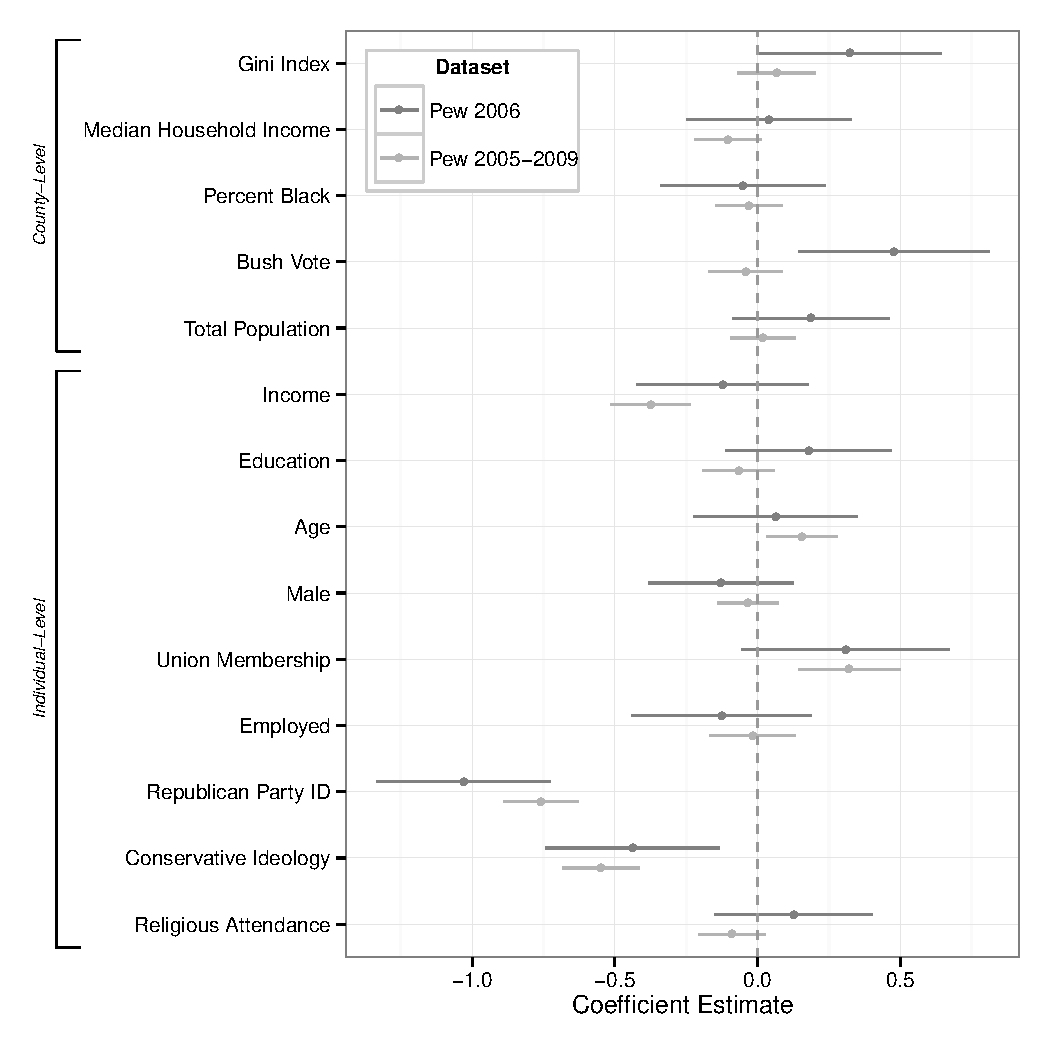
\includegraphics[width=5.25in]{../figures/03_examine_all_available_data_t2.pdf}
  \end{center}
  \begin{footnotesize}
  \begin{tabular}{p{.1in} p{5.1in}}
  & \emph{Notes}: Results from replications of the model presented in Table 2 of \citet{Newman2015} on the 2006 Pew survey analyzed in that article and on pooled data from the six Pew surveys that included the same item and were conducted in the time period the article examines.  The statistically significant result for county income inequality in the 2006 survey presented in that article is not evident when all of the available data are examined.
  \end{tabular}
  \end{footnotesize}
\end{figure}

\begin{figure}[htbp] 
  \caption{Local Inequality and the Perception of America as Divided into `Haves' and `Have-Nots': Results Using Each Available Dataset}
  \label{F:t2_by_survey}
  \begin{center}
    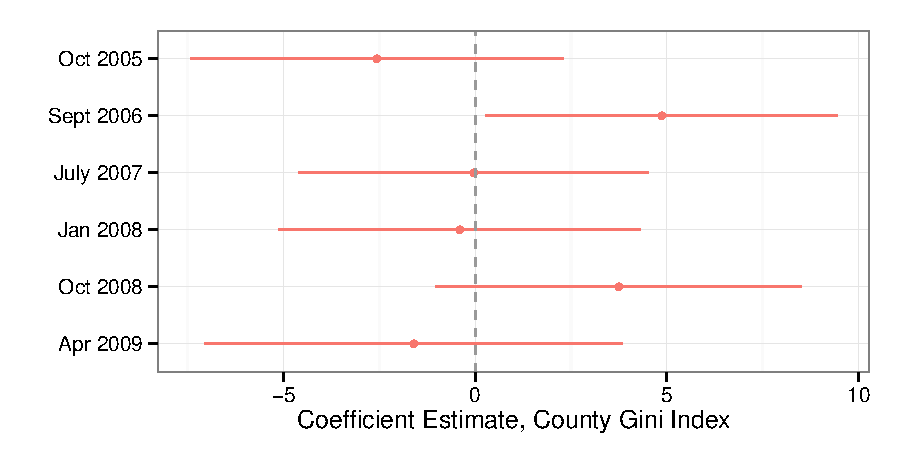
\includegraphics[width=5.25in]{../figures/03_examine_all_available_data_t2_by_survey.pdf}
  \end{center}
  \begin{footnotesize}
  \begin{tabular}{p{.1in} p{5.1in}}
  & \emph{Notes}: Results for county income inequality from replications of the model presented in Table 2 of \citet{Newman2015} on data from each of six available surveys conducted in the in the time period examined in that article.  Of the six surveys, the only one that yields a statistically significant result is the 2006 survey presented in the article.
  \end{tabular}
  \end{footnotesize}
\end{figure}



